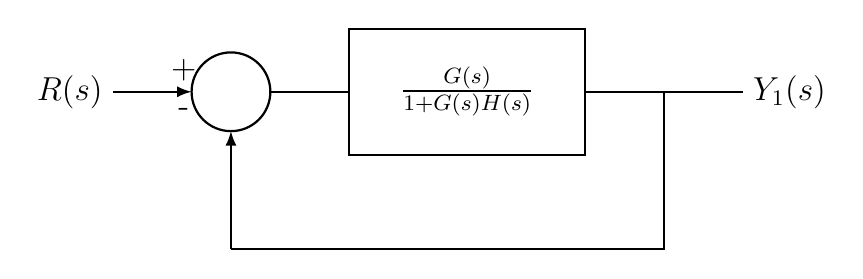
\begin{tikzpicture}[thick,font=\large]
 \draw[-latex] (0,0) -- (1,0);
 \node[left] at (0,0) {$R(s)$};
 \draw (1.5,0) circle [radius=0.5cm];
 \node[above] at (0.9,0){+};
 \node[below] at (0.9,0){-};
 \draw[-] (2,0) -- (3,0);
 \draw (3,-0.8) rectangle (6,0.8);
 \node at (4.5,0){$\frac{G(s)}{1+ G(s)H(s)}$};
 \draw[-] (6,0) -- (8,0);
 \node[right] at (8,0) {$Y_1(s)$};
 \draw[-] (7,0) -- (7,-2) -- (1.5, -2);
 \draw[-latex] (1.5,-2) -- (1.5, -0.5);
\end{tikzpicture}
